\documentclass[9pt]{beamer-control}
\usepackage{beamer-control-prac}
\begin{document}
	
	\TOPIC[1]{System Response}
	\CONCEPT[2]{Week 2: Characterising and modelling systems}

\begin{frame}
\frametitle{Introduction}
In this practical, you will learn how to derive a first-principles model of the inertia disk plant as well as how to characterise its output response.

\vfill

This practical will consist of the following parts:
\begin{itemize}
\item First-principles modelling
\item Characterising the output response
\end{itemize}
\end{frame}


\SUBCONCEPT{First-principles modelling}

\begin{frame}{Deriving the model}
We begin by deriving a first principles model of the inertia disk. A schematic diagram of the motor armature circuit is shown below.

\begin{figure}
	\centering
	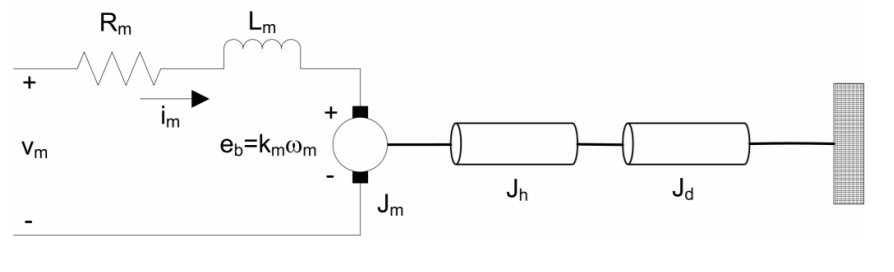
\includegraphics[width=10cm]{prac2_schematic.png}
	\caption{Motor armature circuit schematic diagram.}
\end{figure}
\end{frame}

\begin{frame}{Deriving the model}
The DC motor shaft with moment of inertia $J_m$ is connected to the load hub which is a metal disc used to mount the inertia disc and has a moment of inertia of $J_h$. The back-emf (electromotive) voltage $e_b(t)$ depends on the speed of the motor shaft, $\omega_m$, and the back-emf constant of the motor $k_m$ and opposes the current flow. The back-emf voltage is given by 
\[e_b(t) = k_m \omega _m (t) \]
Using Kirchoff's Voltage Law, we can write
\[v_m(t) - R_m i_m(t)-L_m \frac{\mathrm{d} i_m(t)}{\mathrm{d} t} - k_m \omega_m (t) = 0\]

\end{frame}

\begin{frame}{Deriving the model}
Since the motor inductance $L_m$ is much less than its resistance $R_m$, it can be ignored and we get
\[i_m(t) = \frac{v_m(t) - k_m \omega_m (t)}{R_m} .\]
The motor shaft equation is
\[(J_m+J_h+J_d)\dot{\omega}_m (t) + D_r \omega _m = \tau_m(t)\]
where $D_r$ is the rotor viscous damping coefficient and $\tau_m$ is the applied torque to the DC motor based on the current,
\[ \tau_m(t) = k_m i_m (t).\]
The moment of inertia about the disk can be determined by
\[J_d = \tfrac{1}{2} m_d r_d^2.\]
\end{frame}


\begin{frame}{Deriving the model}
These linear differential equations can be assembled in a state space representation as 
\[\dot{\mathbf{x}} =\mathbf{A}\mathbf{x} + \mathbf{B} \mathbf{u} \quad \text{and} \quad \mathbf{y} =\mathbf{C}\mathbf{x} + \mathbf{D} \mathbf{u} \quad \]	
where the state and output vectors are
\[\mathbf{x} = \begin{bmatrix}
\theta_m \\ \omega_m
\end{bmatrix}
\quad \text{and} \quad \mathbf{y} = \theta_m .\]
Setting the input as $\mathbf{u}=v_m$, the matrices are
\[
\mathbf{A}=\begin{bmatrix}
	0 & 1 \\
	0 & -\left(\tfrac{R_m D_r + k_m^2}{R_m(J_m+J_h+J_d)}\right)
\end{bmatrix},
\mathbf{B} = \begin{bmatrix}
	0 \\ \tfrac{k_m}{R_m(J_m+J_h+J_d)}
\end{bmatrix}, 
\mathbf{C} = \begin{bmatrix}
	1 & 0
\end{bmatrix},
\mathbf{D} = \begin{bmatrix}
	0
\end{bmatrix}
\]  
\end{frame}

\begin{frame}{Simulating the model}
The required parameter values for the QUBE inertia disk are $R_m=8.4\Omega$, $k_m=0.042$ V/(rad/s), $D_r=2\times 10^{-5}$ N.m.s/rad, $J_m = 4\times 10^{-6}$ kg.m$^2$, $J_h = 0.65 \times 10^{-6}$ kg.m$^2$, $m_d=0.053$ kg, and $r_d = 0.0248$ m.

Using these values
\begin{enumerate}
	\item Define the matrices $\mathbf{A}$, $\mathbf{B}$, $\mathbf{C}$, and $\mathbf{D}$ in Matlab 
	\item Use the code on the following slide to set up the state space model in Matlab
	\item Run the code to simulate the systems reponse to a step input 
\end{enumerate}

\end{frame}

\begin{frame}{Simulating the model}
\includematlab{prac1.m}{part1}
\end{frame}


\begin{frame}{Simulating the model}
Similarly, we can use Simulink to simulate the state space model.
\begin{enumerate}
	\item Create a state-space block in Simulink and use the $\mathbf{A}$, $\mathbf{B}$, $\mathbf{C}$, and $\mathbf{D}$ matrices as defined by your Matlab script (Simulink can use these matrices if they are in your Matlab workspace)
	\item Input the same step input into the state-space block as the real plant and connect the output to the same scope
	\item Run the Simulink model and compare the model with the physical plant
\end{enumerate}

What do you notice?

\end{frame}


\begin{frame}{Simulating the model}
	 \begin{figure}
		\centering
		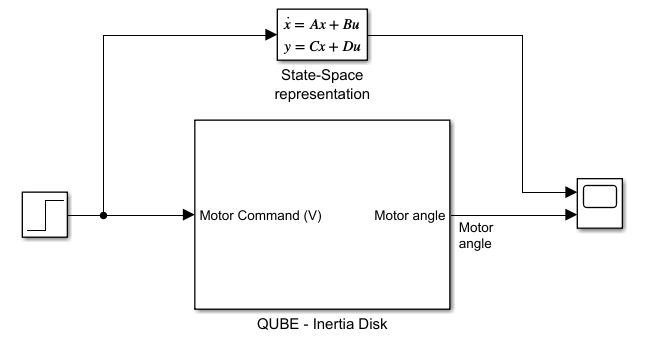
\includegraphics[width=10cm]{prac2_ss_simulink.png}
		\caption{Simulink model with physical plant and state space model.}
	\end{figure}
\end{frame}


\SUBCONCEPT{Characterising the output response}

\begin{frame}{Parameter calculation}
An alternative method to deriving a first principles model is to identify the system by fitting a curve to the output response. 

\begin{itemize}
	\item The open loop (no feedback) response of the inertia disk may be modelled as an Integrator with Time Delay (ITD) model which requires two parameters, $a$ and $\tau$
	\item The intercept $a$ and the time lag $\tau$ may be calculated according to the definition in the notes (also shown in the following figure)
\end{itemize}


\end{frame}

\begin{frame}{Parameter calculation}
	\begin{figure}
		\centering
		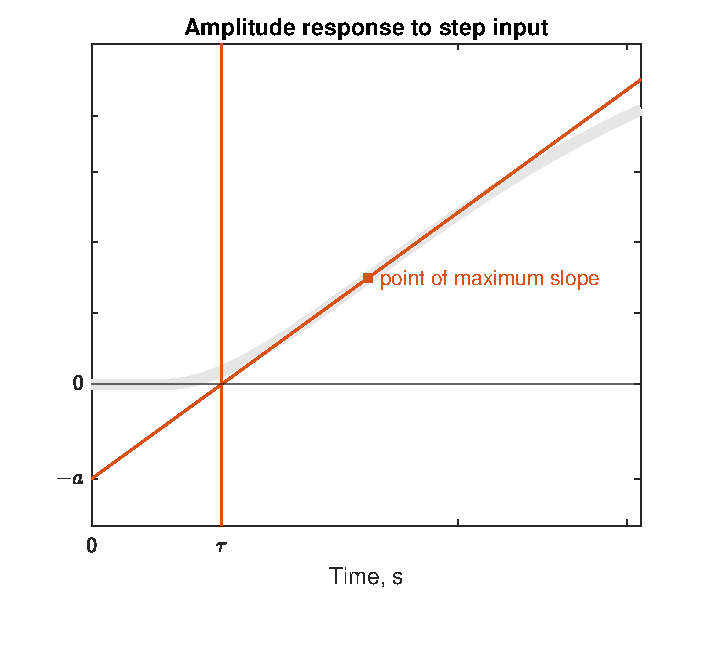
\includegraphics[width=8cm]{itd-at}
		\caption{Integrator with Time Delay (ITD) model.}
	\end{figure}
\end{frame}


\begin{frame}{Characterising the response}
	Approximate the ITD parameters $a$ and $\tau$ of the open-loop inertia disk.
	\begin{enumerate}
		\item Run the Simulink model for 10 seconds to receive the output response to a step input
		\item Open the Scope and click Tools > Measurements > Cursor Measurements to assist in identifying individual points
		\item The vertical lines which appear may be dragged left and right to select points and specific data is given in the Cursor Measurements box on the right of the scope window
		\item Use the following Matlab code to simulate the ITD model
		\end{enumerate}
	\includematlab{prac1.m}{part2}
\end{frame}


\begin{frame}{Next week}
	This week you derived a state-space model of the inertia disk and characterised its output as an ITD model.
		
	When we start looking at controlling a system to reach a desired output we will see that deriving models or characterising output responses give us methods of determining good initial control gains for our controllers. Next week we will be introduced to the concept of feedback to control the inertia disk to reach a desired angle. 
\end{frame}



\end{document}
